\RequirePackage{amsmath}
\DeclareMathOperator*{\argmax}{arg\,max}
\DeclareMathOperator*{\argmin}{arg\,min}

\documentclass{article}

\usepackage[numbers, sort&compress]{natbib}
% \usepackage{pdfpages}
\usepackage{rotating}
\usepackage[margin=1in]{geometry}
\usepackage{graphicx}
\usepackage[strings]{underscore}
\usepackage{anyfontsize}
\usepackage{subcaption}
% \usepackage{lipsum}
\usepackage[toc]{appendix}
% \usepackage[utf8]{inputenc}

\begin{document}


\title{Deep learning emulators of physical simulations for room-scale heat release rate inversion}
\author{}
\date{September 18, 2019}

\maketitle

\begin{abstract}

\end{abstract}




\section{Introduction}
\section{Experimental setup}





\section{Modeling methodology}
\subsection{Overview}

The general approach of the models described in this section is to train on the data acquired from three experimental propane burner fires- hereafter referred to as the training fires. These include two triangle fires, and a symmetric t-squared fire, each with a peak HRR of 200 kW. One triangle fire peaks at 100 seconds from ignition and the other peaks at 300 seconds from ignition. The t-squared fire follows the equation $\dot{Q} = \alpha t^2$ with $\alpha=0.01172$ kW/s$^2$ until the HRR reaches 200 kW. At this point, the HRR is held constant at 200 kW for 50 seconds. Finally, the fire follows an inverted t-squared downward ramp, which produces a symmetric HRR curve. All three fire ramps in the training set are shown in figure \ref{fig:training_ramps}. These fires can be viewed as the experimental calibration for the machine learning models. A test case was also run in order to evaluate the models. This ramp is intended to be relatively dissimilar from those in the training set and to resemble a potential non-idealized HRR curve that could arise in a calorimetry experiment. This curve initially ramps up slowly for about 100 seconds, then ramps up to a peak of 200 kW. It then quickly ramps down to about 50 kW and remains steady for about 200 seconds. Finally it ramps back up to about 90 kW before it is extinguished. This ramp is shown in figure \ref{fig:test_ramp}. When developing the models, only information from the experiments in the training set is used in order to allow for meaningful model evaluation.

\begin{figure}[htbp]
  \centering
  \begin{subfigure}[t]{.45\textwidth}
      \centering
      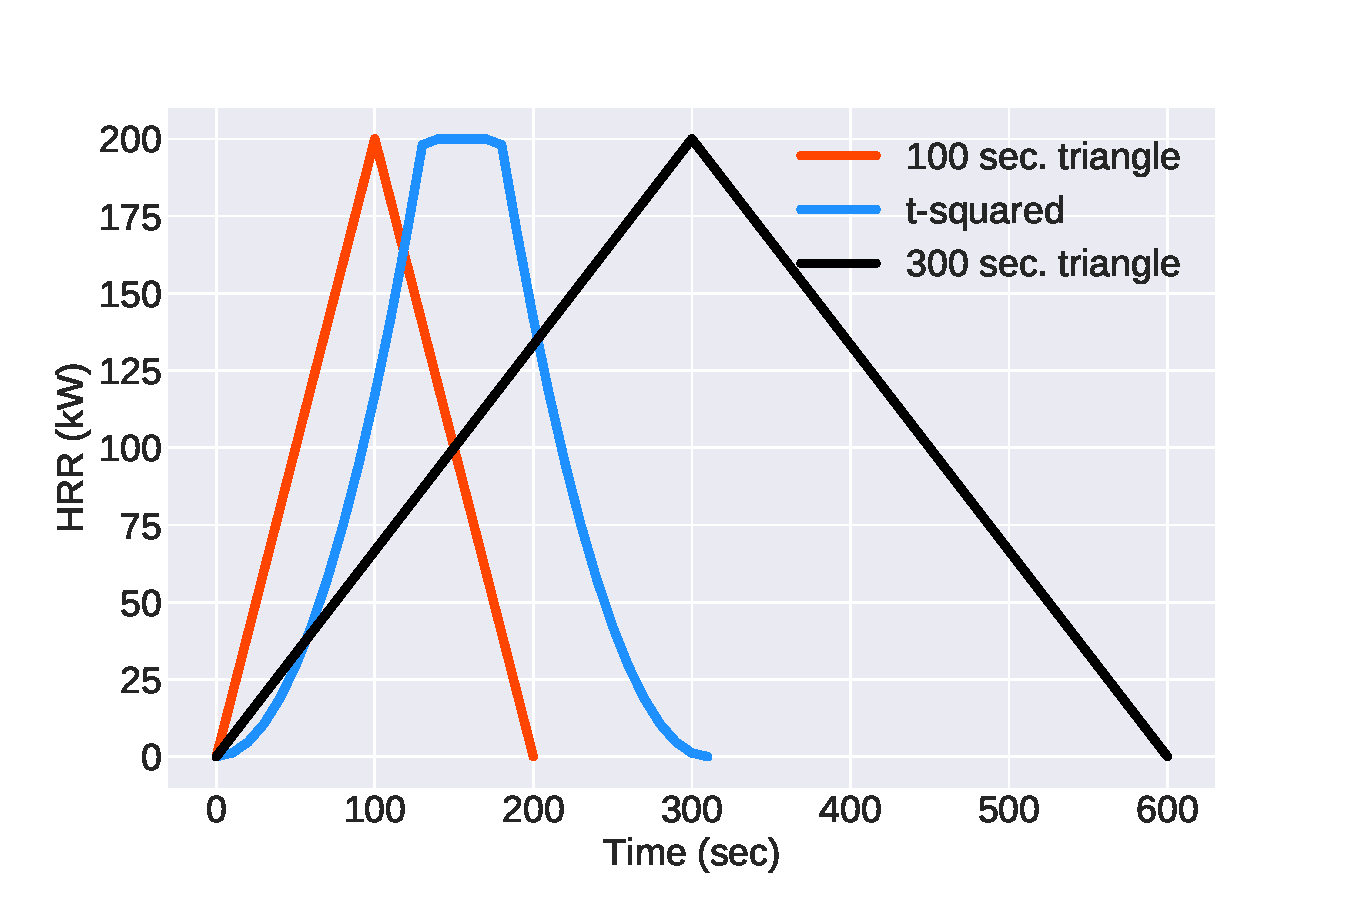
\includegraphics[width=\textwidth,keepaspectratio]{figures/training_ramps.pdf}
      \caption{Training HRR ramps}
      \label{fig:training_ramps}
  \end{subfigure}
  \begin{subfigure}[t]{.45\textwidth}
      \centering
      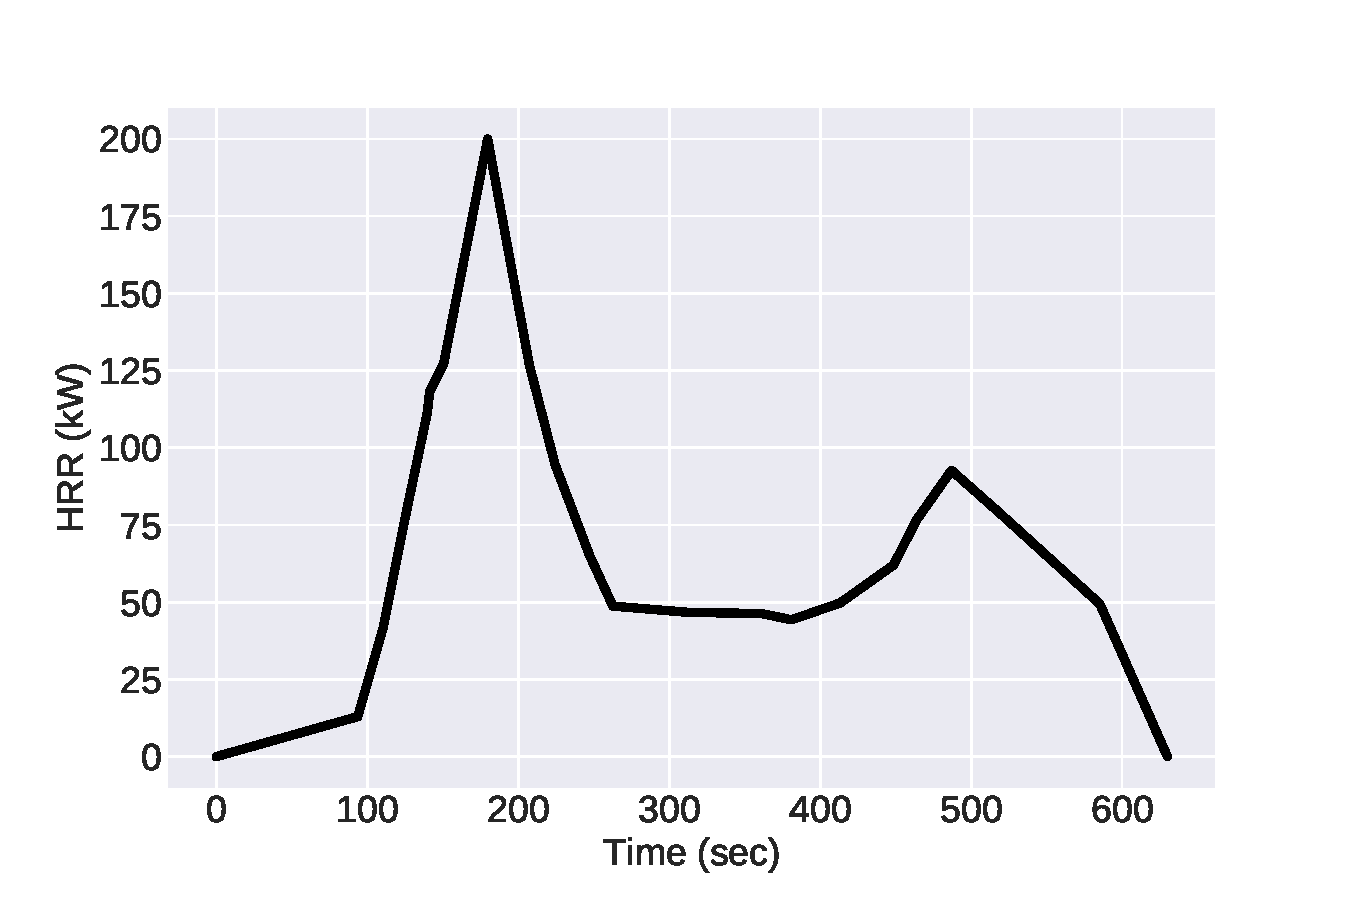
\includegraphics[width=\textwidth ,keepaspectratio]{figures/test_ramp.pdf}
      \caption{Test HRR ramp}
      \label{fig:test_ramp}
  \end{subfigure}
  \caption{\protect\ref{fig:training_ramps} shows the three HRR ramps used in the experiments that comprise the training set for the machine learning models. \protect\ref{fig:test_ramp} shows the HRR ramp used in the experiment that is used to evaluate the models.}
  \label{fig:hrr_ramps}
\end{figure}


\subsection{Heat flux measurements}
This section describes machine learning methods for inferring the heat release rate of a compartment fire using heat flux measurements from the directional flame thermometers (DFTs) of the aforementioned experimental setup. Modak's point source model \cite{modak1977thermal} provides a simple and intuitive relationship between a fire's heat release rate and the resulting incident radiative heat flux on a nearby target. This model assumes that the radiative energy from a fire emanates isotropically from the center of a fire such that the incident radiative heat flux on a target is described by equation \ref{eqn:point_source},

 \begin{equation}
  \label{eqn:point_source}
  q" = \frac{\chi_R\dot{Q}cos\theta}{4\pi R^2}
\end{equation}

where $q"$ is the incident radiative heat flux at a target located at a distance $R$ from the center of the fire, $\chi_R$ is the radiative fraction of the fire, and $\theta$ is the angle between the normal to the surface of the target and the line of sight between the target and the fire. Fleury \cite{fleury2010evaluation} also evaluated six different radiation models against experimental data and found the point source model to be the most accurate. Equation \ref{eqn:point_source} suggests that for a fixed fire location and stationary targets, $\chi_R \dot{Q} \propto q"$. This linear proportionality motivates the use of linear statistical models whose form is specified according to equation \ref{eqn:linear_model}.

 \begin{equation}
  \label{eqn:linear_model}
  \chi_R  \boldsymbol{\dot{Q}} = \boldsymbol{q}" \beta + \boldsymbol{\epsilon}
\end{equation}

For and experiment with $n$ observations and $m$ DFTs, $\boldsymbol{\dot{Q}} \in  \textbf{R}^n$ is a vector of HRR values, $\boldsymbol{q}" \in \textbf{R}^{n\text{x}m}$ is a matrix of heat flux measurements, $\beta \in \textbf{R}^n$ is a vector of regression slopes, and $\boldsymbol{\epsilon} \in \textbf{R}^n$ is vector of random errors. Note that equation \ref{eqn:linear_model} assumes that $\chi_R$ is constant throughout an experiment; it is not necessarily constant across different experiments if different fuels are used. Also, if only one DFT were used, the point source model would suggest that $\beta = \frac{4 \pi R^2}{ cos \theta}$. However, this is not true for the multivariate case, and as a result, the coefficients of $\beta$ are instead learned from the experimental data. 

In addition to the theoretical explanation from Modak's point source model, the scatterplots shown in Figure \ref{fig:dft_scatterplot} show the linear relationship between $\boldsymbol{\dot{Q}}$ and $\boldsymbol{q}"$ from the training set experiments. 

\begin{figure}[htbp]
  \centering
  \begin{subfigure}[t]{.45\textwidth}
      \centering
      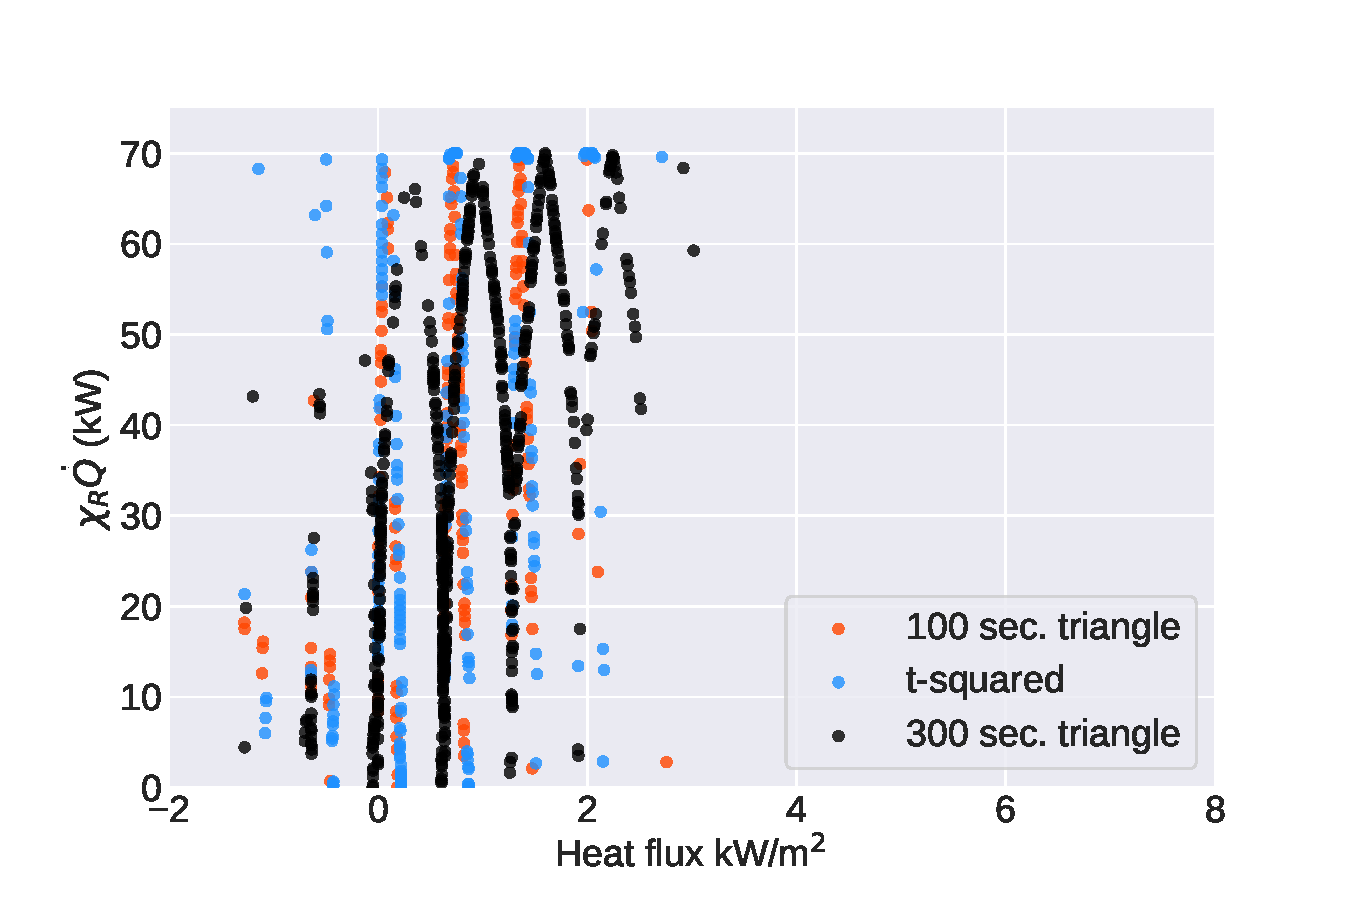
\includegraphics[width=\textwidth,keepaspectratio]{figures/weak_dft_scatter.pdf}
      \caption{Weak correlation}
      \label{fig:weak_scatter}
  \end{subfigure}
  \begin{subfigure}[t]{.45\textwidth}
      \centering
      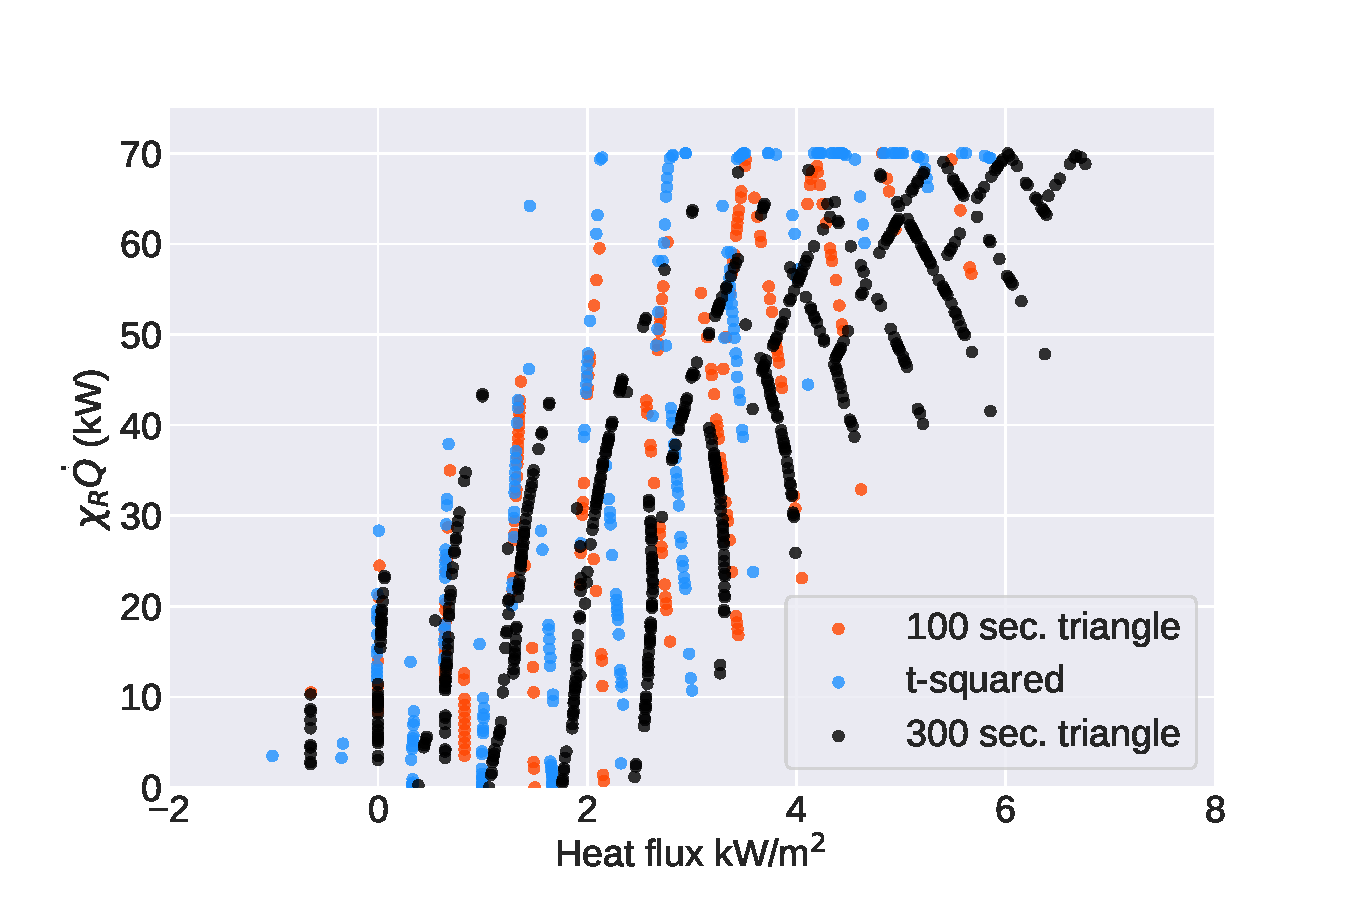
\includegraphics[width=\textwidth ,keepaspectratio]{figures/moderate_dft_scatter.pdf}
      \caption{Moderate correlation}
      \label{fig:moderate_scatter}
  \end{subfigure}
   \begin{subfigure}[t]{.45\textwidth}
      \centering
      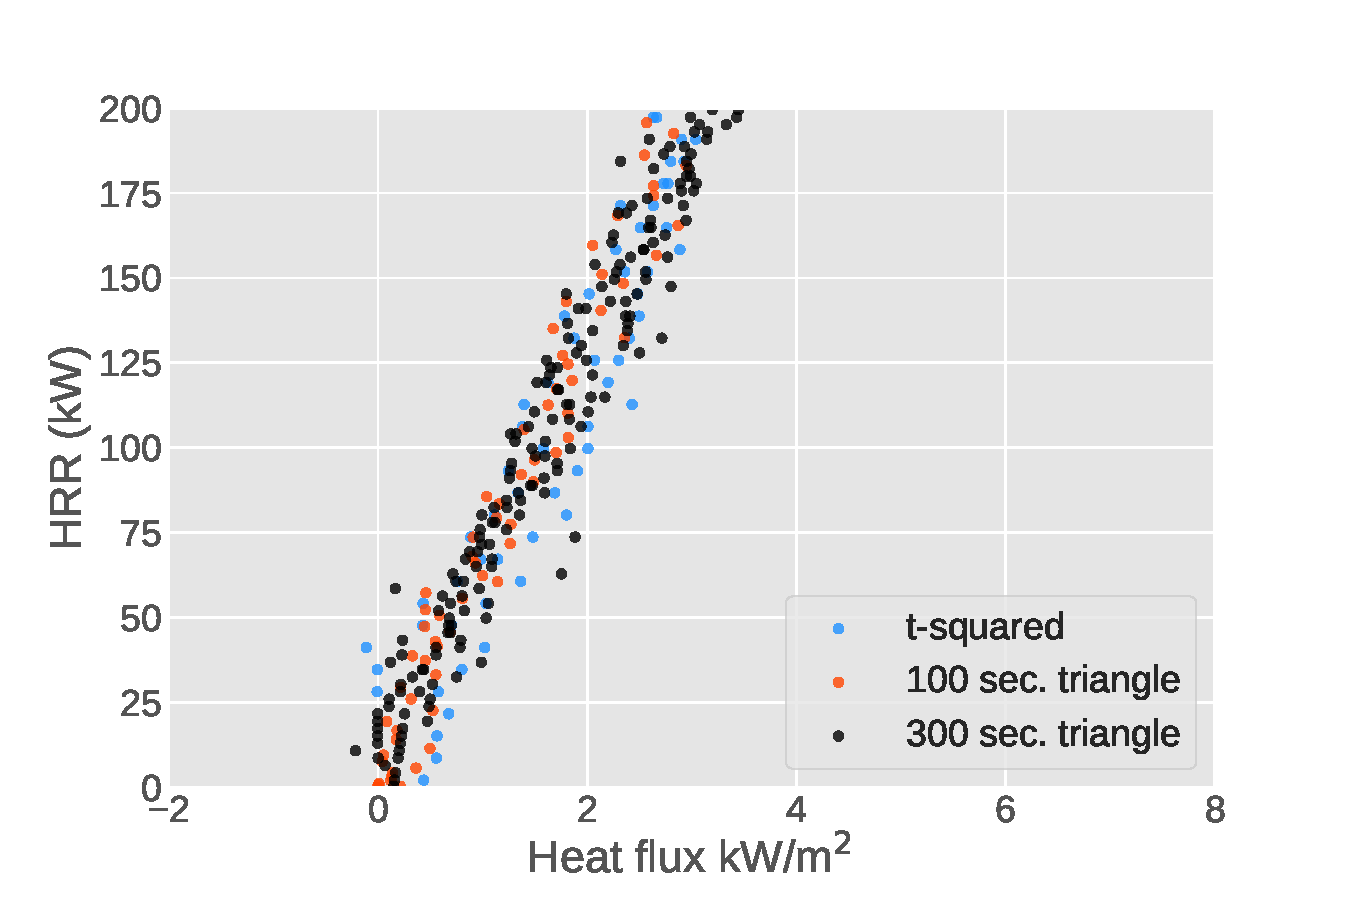
\includegraphics[width=\textwidth ,keepaspectratio]{figures/strong_dft_scatter.pdf}
      \caption{Strong correlation}
      \label{fig:strong_scatter}
  \end{subfigure}
  \caption{Scatterplots of the radiative heat release rate vs. measured heat flux for three different DFTs. These examples demonstrate the variation in the strength of correlations across DFTs.} 
  \label{fig:dft_scatterplot}
\end{figure}

The examples shown in Figure \ref{fig:dft_scatterplot} demonstrate how the strength of the correlation between the radiative HRR and measured heat flux varies significantly across the different DFTs. This finding raises several questions regarding the design of the model. First, should all the DFTs be included in the model? If not, which ones should be excluded and why? It may seem that the best set of sensors to include in the model is the one that includes only the DFTs whose measured heat flux is the most correlated with the radiative heat release rate. However, this is not necessarily true because multiple DFTs with strong correlations can provide redundant information. 

To circumvent these issues, a lasso regression is employed. This technique is a modified linear regression that performs feature selection in addition to estimating values of $\beta$. These values are estimated according to equation \ref{eqn:lasso}:

 \begin{equation}
  \label{eqn:lasso}
  \hat\beta_{lasso} = \argmin_{\beta}\Bigg\{ \underbrace{\big[\chi_R \boldsymbol{\dot{Q}} - \boldsymbol{q}" \beta\big]^T\big[\chi_R \boldsymbol{\dot{Q}} - \boldsymbol{q}" \beta\big]}_{\text{I}} + \underbrace{\lambda||\beta||_1}_{II}   \Bigg\}
\end{equation}

\noindent where $||\beta||_1$ is the $l^1$ norm of $\beta$ and $\lambda$ is a hyperparameter that is learned from the data. Note that term I is simply the sum of the squared residuals, meaning that if term II is zero, the process is identical to a ordinary least squares linear regression. The inclusion of term II, also known as L1 regularization, serves two purposes. First, it helps prevent overfitting as term II can be viewed as a penalty for increased model complexity. Second, it performs feature selection as L1 regularization has a tendency to set values in $\beta$ to zero, thereby removing the corresponding feature from the model. It should be noted that the use of the $l^2$ norm (known as ridge regression) is another common technique to combat overfitting; however, unlike lasso regression, ridge regression does not also perform feature selection. 


\begin{figure}[htb] \centering
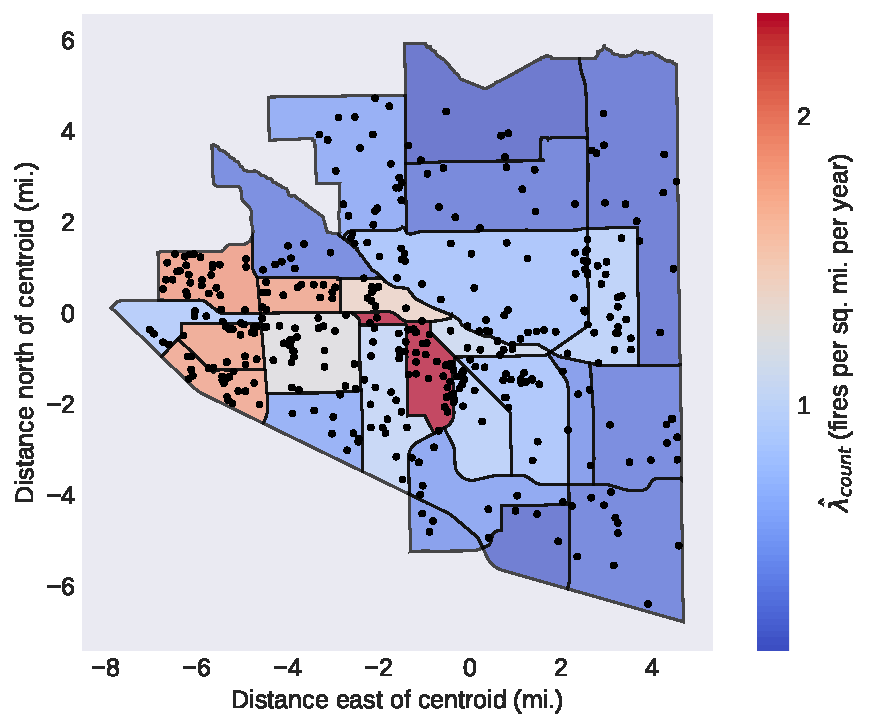
\includegraphics[width=.75\textwidth]{./figures/spatial_histogram.pdf}
\caption{A visual depiction of the naive count forecasting methodology for an example department. Each black dot marker indicates the location of a residential fire that occurred during the six-year training interval, 2006-2011 (inclusive). The color of a tract corresponds to the fire count density rate estimated from this approach for that tract. Notice that large census tracts with few fires have the lowest density rate and small tracts with many fires have the highest density rate.}
\label{fig:spatial_histogram}
\end{figure}




\clearpage
\bibliographystyle{unsrtnat}
\bibliography{./references.bib}
\end{document}
